%%%%%%%%%%%%%%%%%%%%%%%%%%%%%%%%%%%%%%%%%%%%%%%%%%%%%%%%%%%%%%%%%%%%%%%%%%%%%%%%
%
% File:   archaeopteryx.tex
% Author: Sudnya Diamos
%         Gregory Diamos
% Date:   Saturday September 3, 2011
% Brief:  The latex source file for the Archaeopteryx simulator paper.
% 
%%%%%%%%%%%%%%%%%%%%%%%%%%%%%%%%%%%%%%%%%%%%%%%%%%%%%%%%%%%%%%%%%%%%%%%%%%%%%%%%

%\documentclass[12pt]{report}
\documentclass[conference, 10pt]{IEEEtran}

%%%%%%%%%%%%%%%%%%%%%%%%%%%%%%%%%%%%%%%%%%%%%%%%%%%%%%%%%%%%%%%%%%%%%%%%%%%%%%%%
% Included Packages
\usepackage{cite} 
\usepackage[pdftex]{graphicx} 
\usepackage{url}
\usepackage{booktabs} 
\usepackage{setspace}
%%%%%%%%%%%%%%%%%%%%%%%%%%%%%%%%%%%%%%%%%%%%%%%%%%%%%%%%%%%%%%%%%%%%%%%%%%%%%%%%

%%%%%%%%%%%%%%%%%%%%%%%%%%%%%%%%%%%%%%%%%%%%%%%%%%%%%%%%%%%%%%%%%%%%%%%%%%%%%%%%
% Configure Document
\topmargin      0.0in
\headheight     0.0in
\headsep        0.0in
\oddsidemargin  0.0in
\evensidemargin 0.0in
\textheight     9.0in
\textwidth      6.5in
%%%%%%%%%%%%%%%%%%%%%%%%%%%%%%%%%%%%%%%%%%%%%%%%%%%%%%%%%%%%%%%%%%%%%%%%%%%%%%%%

%%%%%%%%%%%%%%%%%%%%%%%%%%%%%%%%%%%%%%%%%%%%%%%%%%%%%%%%%%%%%%%%%%%%%%%%%%%%%%%%
% Configure Packages
\graphicspath{{images/}} 
\DeclareGraphicsExtensions{.pdf,.jpeg,.jpg,.png} 
\pagenumbering{arabic}
%%%%%%%%%%%%%%%%%%%%%%%%%%%%%%%%%%%%%%%%%%%%%%%%%%%%%%%%%%%%%%%%%%%%%%%%%%%%%%%%

%%%%%%%%%%%%%%%%%%%%%%%%%%%%%%%%%%%%%%%%%%%%%%%%%%%%%%%%%%%%%%%%%%%%%%%%%%%%%%%%
%% New Commands
%%%%%%%%%%%%%%%%%%%%%%%%%%%%%%%%%%%%%%%%%%%%%%%%%%%%%%%%%%%%%%%%%%%%%%%%%%%%%%%%

%%%%%%%%%%%%%%%%%%%%%%%%%%%%%%%%%%%%%%%%%%%%%%%%%%%%%%%%%%%%%%%%%%%%%%%%%%%%%%%%
% High Level Organization (See individual sections for details) - 8000 words
% 
% Chapter 1) - Introduction                            - 1000 words
% Chapter 2) - Vanaheimr introduction                  - 500  words
% Chapter 3) - Executive Summary (emphasis on speedup) - 750  words
% Chapter 4) - Framework Design                        - 1750 words
% Chapter 5) - Simulator Core Design                   - 3000 words
% Chapter 6) - Experimental Evaluation                 - 1000 words
% Chapter 7) - Related Work                            - 500  words
% Chapter 8) - Conclusions                             - 500  words
%
%%%%%%%%%%%%%%%%%%%%%%%%%%%%%%%%%%%%%%%%%%%%%%%%%%%%%%%%%%%%%%%%%%%%%%%%%%%%%%%%

\begin{document} 

%%%%%%%%%%%%%%%%%%%%%%%%%%%%%%%%%%%%%%%%%%%%%%%%%%%%%%%%%%%%%%%%%%%%%%%%%%%%%%%%
% Title and Authors
\title{Archaeopteryx\\
A Multi-BSP Processor Simulator}

\author{Sudnya Diamos and Gregory Diamos  \\
No Affiliation \\
{\small mailsudnya@gmail.com, gregory.diamos@gatech.edu}}
\date{\today}

\maketitle
%%%%%%%%%%%%%%%%%%%%%%%%%%%%%%%%%%%%%%%%%%%%%%%%%%%%%%%%%%%%%%%%%%%%%%%%%%%%%%%%

%%%%%%%%%%%%%%%%%%%%%%%%%%%%%%%%%%%%%%%%%%%%%%%%%%%%%%%%%%%%%%%%%%%%%%%%%%%%%%%%
% Section 1 - 1000 words
\section{Introduction}
\label{sec:introduction}

% Survey of the space
The transition to many core computing has coincided with the growth of
data parallel computation and the evolution of graphics processing
units (GPUs) from special purpose devices to programmable cores. 
The emergence of low cost programmable GPU computing substrates from
NVIDIA, Intel, AMD, and ARM have made data parallel architectures commodity
from embedded systems through large scale clusters such as the
Tsubame~\cite{ref:tsubame} and Keeneland systems~\cite{ref:keeneland}
hosting thousands of GPU chips.

The dominant programming systems involve the use of
bulk-synchronous-parallel programming models~\cite{ref:bulk-synchronous}
embodied by languages such as CUDA, OpenCL, and C++-AMP.  These data-parallel
languages implement \textit{single instruction stream multiple thread} (SIMT)
models of computation that specify a large number of
data-parallel threads that can be readily exploited by hardware
multi-threading and \textit{single-instruction-multiple-data} (SIMD)
cores. 

In contrast to many-core processors based on out-of-order CPU cores,
GPU architectures are designed to exploit the massive data-parallelism of
bulk-synchronous programs. Performance is maximized for regular computations
where hardware can use SIMD pipelines and bulk data transfers to exploit
control and data locality among threads.  However, current designs suffer
from steep performance cliffs when executing programs with irregular control
flow and data access patterns.  
%from branch divergence (when threads take
%different paths through the program) and memory divergence (when threads perform
%scatter or gather memory accesses).  
They are also beginning to introduce new
programming hazards as they move to \textit{non-uniform memory access} (NUMA)
organizations to reduce on-chip network overheads.  

These performance hazards limit the potential of GPU programming. In fact,
sequential algorithms mapped to single CPU cores are still competitive with GPUs
for many application domains (e.g. database queries, loss-less compression,
lexing/parsing, or graph analytics) despite a 300x (and exponentially growing)
difference in peak throughput.  Two of the most important problems in computing
today involve designing architectures with more gradual performance cliffs
(without sacrificing parallel efficiency), and
designing bulk-synchronous algorithms for irregular applications.  

% attention grabber
Unfortunately, the tools that have been traditionally used to explore solutions
to these problems (architecture simulators and analytical models) fall into the
category of applications \textit{without} efficient parallel implementations. 
This has created a gap between parallel processor and simulator performance that
is widening with each successive generation, limiting the ability of architects
to explore the design space of possible optimizations and the ability of
application designers to evaluate the impact of algorithms on future
architectures.  

% Functional modeling
This is even more troubling for functional verification.  Although most bugs are
still caught with relatively short directed tests~\cite{ref:bug-distributions},
a critical class of bugs only occurs during complex interactions between
multiple components.  These bugs are typically discovered through application
stress testing or random program execution.   As application complexity
continues to grow with processor capability, there is a rising concern that
simulator performance will limit application and random test coverage,
especially for applications with multiple phases.  

% Why are we doing this?
It would be desirable to leverage the tremendous growth in computing potential
provided by parallel processors for microarchitecture simulation.  However,
the sequential operation and tight dependency loops in high performance 
processor pipelines quickly dash the hopes of straightforward solutions.
Exploiting fine-grained data parallelism and expressing the operation of a
processor in terms of hierarchical bulk data transfers requires a ground-up
approach.

% Our approach
In this paper, we assert that the parallel and hierarchical organization of
microarchitecture structures used in modern processors provide a natural
basis for simulation using data-parallel algorithms.  We test this assertion by
implementing a composable functional simulator for a new processor architecture,
and then augment it with performance models for key micro-architecture
structures.  We exploit fine-grained data parallelism by using hundreds of
threads to simulate a single core.  We show how basic parallel algorithm
building blocks like reductions, prefix sums, sorts, and histograms can be used
to simulate instruction fetch units, register files, thread schedulers,
functional units, and caches.  Across X applications, we show that the accuracy
of the simulation is comparable to state-of-the-art sequential simulators, and
that the performance of the simulator scales across three generations of GPUs.
This paper describes the first data-parallel processor simulator that can 
leverage the technology scaling and microarchitecture enhancements of the
previous generation of GPU hardware to simulate the next.

% Contributions
Specifically, this paper makes the following contributions:

\begin{itemize}
	\item It describes the design of the first processor simulator implemented
		completely in the CUDA "C" language.

	\item It introduces a design methodology for simulating parallel processors
		that achieves near peak utilization of modern GPU accelerators and
		good scaling across three generations of GPUs.
		
	\item It shows that microarchitecture details, such as scratchpad sizes,
		hardware thread schedulers, register file organizations, cache
		hierarchies, and core pipelines can be simulated quickly as long as
		the hierarchical organization of the machine is maintained.
	
	\item It compares the results and performance of our parallel simulator with
		two existing GPU simulators: GPGPU-Sim, and the Ocelot PTX Emulator.  
		We demonstrate a Nx speedup.
\end{itemize}

\subsection{Outline}

This document is organized as follows.  
Section~\ref{sec:vanaheimr} briefly describes the processor being simulated.
Section~\ref{sec:summary} walks through the execution of sample application on
the proposed simulator.
Section~\ref{sec:framework-design} provides a high level overview of the 
simulator framework. 
Section~\ref{sec:core-design} drills down into the implementation details of 
the simulator.  
This is followed by Section~\ref{sec:experiments}, which provides an evaluation
of the speed and accuracy of the simulator.
Section~\ref{sec:related-work} surveys related work, and
Section~\ref{sec:conclusion} concludes the paper.

%%%%%%%%%%%%%%%%%%%%%%%%%%%%%%%%%%%%%%%%%%%%%%%%%%%%%%%%%%%%%%%%%%%%%%%%%%%%%%%%

%%%%%%%%%%%%%%%%%%%%%%%%%%%%%%%%%%%%%%%%%%%%%%%%%%%%%%%%%%%%%%%%%%%%%%%%%%%%%%%%
% Section 2 - 500 words
\section{Vanaheimr}
\label{sec:vanaheimr}

Vanaheimr is an architecture that is optimized to execute Multi-BSP programs
that express a high degree of parallelism hierarchically.  The memory system
is composed of memory controllers that are tiled across the processor die
and connected to 3D DRAM modules either directly through vias, or
indirectly through a silicon interposer.  The cache is organized
into an H-tree structure, with clusters at each level of the hierarchy.  Each
level is connected by a stage of an indirect network.  The cache bank size,
number of levels, as well as degree of connectivity at each level is
configurable.  

The cores themselves implement a hierarchical SIMD architecture.
The main difference between this and a traditional SIMD processor is that the
unit of control that is broadcast to multiple execution units is larger than
a single instruction; it is referred to as a sub-kernel.  Cores may be
heterogeneous at the micro-architecture level to balance sequential against
parallel efficiency.  However, they all implement the same ISA and execution 
model. The architecture is intended to scale across regular and irregular 
applications by varying the ratio of execution units to memory, and the number 
of levels in the interconnection network.  

This paper is concerned with the design of a functional simulator for the
Vanaheimr architecture, so only the essential aspects are mentioned here. 
Additional details about the architecture are described in related
work~\cite{ref:vanaheimr}.  

\subsection{Architecture}
Vanaheimr targets 100 TFLOPs peak throughput at a 5nm technology node on a
300mm$^2$ die, while peak single-threaded CPU performance is currently limited
to less than 15 GFLOPs~\cite{ref:sandybridge-peak}.  In order to bridge the gap
between simulator and hardware performance, the Archaeopteryx simulator is
implemented using Multi-BSP algorithms that are intended to execute on a
commodity parallel processor, such as NVIDIA Kepler with a peak throughput of
2.5 TFLOPs (GK104) or greater.

Although some components, namely the SIMD lanes, used in the Vanaheimr
architecture map naturally onto the CUDA model, the memory system, network,
and core control logic exhibit either serial operation in hardware or many
fine-grained dependences.  These components are modeled individually by
leveraging bulk-parallelism where it exists (such as among network buffers and
lanes), and falling back to serial execution where it does not (such as the
SIMD instruction fetch to broadcast loop). Individual components are composed 
together hierarchically into levels in the final Multi-BSP simulation that
expand or contract the amount of parallelism during execution.  

\subsection{Programming Model}
Vanaheimr programs are compiled into an intermediate form, VIR (the Vahanheimr
Internal Representation), from a high level language such as CUDA with nested
parallelism, OpenCL, Phalanx, Sequoia, or any other that can be mapped onto
the Multi-BSP model. VIR is a RISC-like instruction set that shares many opcodes
and the type system with LLVM.  However, it also defines a flexible mechanism
for declaring scratchpad memory that is shared at different levels in a 
hierarchical thread array (HTA).  

During compilation, a program is first lowered into VIR, where device agnostic
optimizations are applied. Then, a device-specific backend transforms the code
to conform to the machine ABI for function calls and variable layout in memory. 
It also translates VIR opcodes into machine instructions and performs scheduling
and resource allocation of memory, registers, and code.  A final binary is
produced that is suitable for execution in a SPMD fashion.

% Kernel Launch
%  - synchronous
%  - asynchronous
Programs begin with a single thread entering a \textit{main} function.  This
thread may perform scalar operations, or make system calls to allocate memory or
interact with IO devices; it may also create additional threads by launching a
HTA.  HTAs can be launched synchronously or asynchronously.  Synchronous
launches suspend the calling thread until the HTA returns, while asynchronous
launches create a continuation that launches the HTA after the current thread
finishes.  Parallelism can be specified statically via the launch of a single
multi-level HTA, or it can be created dynamically, via the recursive launch of
many HTAs with fewer levels.  This allows regular applications to avoid the
overheads of runtime work creation, and irregular applications to adjust the
amount of parallelism to match the shape of data-dependent problems.

% Memory allocation
%  - static
%  - dynamic
Memory allocation is performed statically with automatic variables, or
dynamically via a malloc equivalent.  The main difference between these concepts
and their sequential counterparts is that they also specify the level in the HTA
at which they are replicated.  For example, a statically sized array of integers
could be allocated per-thread, once for the entire HTA, or replicated at any
other level.  Similarly, a call to malloc could be made by each thread to
allocate memory to store a private data structure, or by a single-thread to
allocate memory that is shared across threads at the same level.  
The exact mechanism used to specify the scope of a variable is left to the 
programming language designer.  This mechanism is meant to communicate this 
information to the runtime or compiler, which can control the placement of these
memory allocations at the appropriate level in the memory hierarchy.

% Synchronization
%  - barriers
%  - call-return
Synchronization can be performed explicitly via barriers at any level of a HTA,
or implicitly through the bulk-synchronization mechanism as HTAs complete.  This
means that memory that was modified by a synchronously launched HTA will be 
immediately available to the calling thread when it resumes.  


%%%%%%%%%%%%%%%%%%%%%%%%%%%%%%%%%%%%%%%%%%%%%%%%%%%%%%%%%%%%%%%%%%%%%%%%%%%%%%%%

%%%%%%%%%%%%%%%%%%%%%%%%%%%%%%%%%%%%%%%%%%%%%%%%%%%%%%%%%%%%%%%%%%%%%%%%%%%%%%%%
% Section 2 - 750 words
\section{Executive Summary}
\label{sec:summary}

This paper begins with a concrete example of the simulation of single
application on an instance of the Vanaheimr processor architecture.  

\subsection{Application Overview}

%%
%% Saxpy figure
%%
\begin{figure}
	\begin{center}
		%% TODO replace with real image
		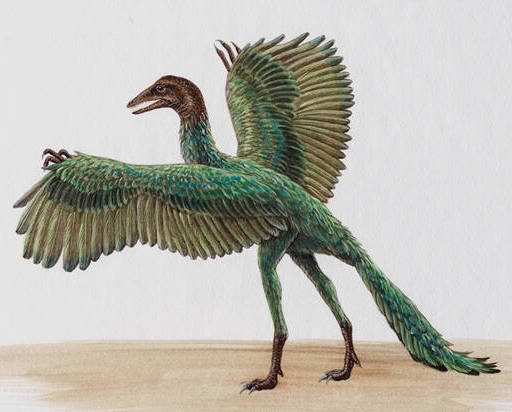
\includegraphics[width=0.9\linewidth]{archaeopteryx-bird}
		\caption{The SAXPY kernel CUDA "C" source code.}
		\label{fig:saxpy-kernel-source}
	\end{center}
\end{figure}

SAXPY is the canonical example of a data-parallel program from the dense linear
algebra application domain.  A single multiply-accumulate kernel is applied to
each element in a one-dimensional vector.  The CUDA C source code for this
kernel is shown in Figure~\ref{fig:saxpy-kernel-source}.

%%
%% Main thread figure
%%
\begin{figure}
	\begin{center}
		%% TODO replace with real image
		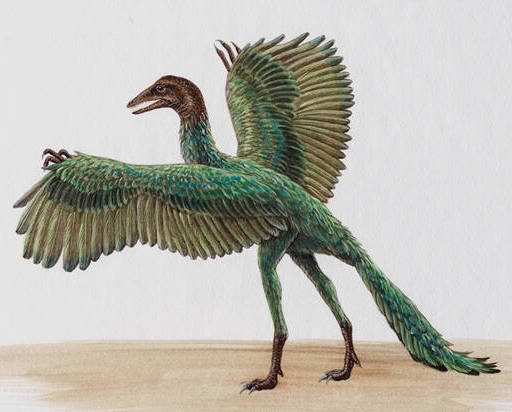
\includegraphics[width=0.9\linewidth]{archaeopteryx-bird}
		\caption{The main program thread CUDA "C" source code.}
		\label{fig:saxpy-main-thread}
	\end{center}
\end{figure}

% Data distribution, initialized randomly
The program begins with a single thread, which allocates the X and Y arrays,
then initializes them with random data.  It then applies a block-cyclic
data-distribution to the X and Y arrays, which partitions them into contiguous
blocks that are allocated on the same DRAM module, managed by the same memory
controller, and processed by the same core.  Once memory has been initialized,
the main thread launches the SAXPY kernel synchronously, expanding the amount
of parallelism.  The dimensions of the input and output data sets are known
statically, as are the elements from each set that will be processed by each
thread.  This simplifies the problems of creating data distributions and HTAs,
and they can be created at once when the kernel is launched.  More complex
applications may require creating additional HTAs or changing data distributions
during kernel execution.  However, the simple example of SAXPY is covered first.  

Once the kernel returns control transfers back to the main thread and
memory is synchronized, the results are verified, memory is freed, and the
program exits.  

% Data distributions - detail
Although SAXPY is a completely data-parallel algorithm with one operation
naturally mapping onto a single thread, the kernel is composed of a two-level
hierarchy of thread arrays, with each array containing several hundred threads.
This is done to reduce the overhead of launching individual threads, and to
coarsen the granularity of the input and output data distributions.  This
coarsening eases the process of mapping thread arrays to cores with good data
locality.

% Kernel execution, a two-level HTA mapped onto cores
The kernel launch specifies the dimensions of the HTA as well as the input
parameters to the kernel.  A two-level HTA is created.  The first level is an
array of 1024 threads and the second level is an array of arrays that covers
the entire input and output data sets.  No scratchpad memory is allocated since
this application simply reads an input and writes an output without any reuse
or any inter-thread communication.  The kernel parameters (pointers to the X, Y
arrays and the value of A) are broadcast to each thread; they are initialized
before the thread is created.  After it has been created, each thread determines
its id, finds the offset of the elements in X and Y that it should process,
performs the $Y = A*X+Y$ calculation, and exits.

\subsection{Compilation}

In order to execute Vanaheimr programs such as SAXPY on the Archeopteryx
simulator, they must be compiled into the VIR form from source.  

% Programming model changes
Vanaheimr's programming model extends the baseline defined by CUDA "C" in
several ways, for example, by allowing device threads to call CUDA API routines,
and by extending the two-level CUDA kernel to an HTA with unbounded levels.

% Main thread example

% Example inner loop (kernel) of saxpy

% Mapping into VIR 
%% - show C line to instruction translation
The mapping from CUDA "C" into VIR is performed in a straightforward manner.
NVIDIA's CUDA compiler is used as a frontend to lower the C-like language into
a virtual assembly language, PTX.  A modified version of the Ocelot compiler is
then used transform PTX into VIR.  During this process, several PTX intrinsics
for launching HTAs, declaring statically allocated variables with specific
HTA-level scoping, and dynamically allocating scratch-pad memory are recognized
as PTX intrinsic functions and converted into VIR abstractions.  These
abstractions can be analyzed and optimized by the VIR optimizing compiler, which
is also written in CUDA.

%% - show parameter memory passing
%% Parameters
Kernel parameters are declared explicitly in VIR in kernel definitions. 
For example, the VIR representation of the SAXPY kernel in 
Figure~\ref{fig:saxpy-vir} includes the variables X, Y, and A in the kernel
prototype.  These parameters are accessed via explicit load
instructions in the kernel body. In a real implementation, these parameter
accesses would be either converted into reads from pre-initialized registers or
loads from memory by a backend compiler for Vanaheimr.  However, since this
form of the program is simulated directly, they are supported by the simulator
and complete in a single instruction.

% - show data distribution, per-thread group
As simulated HTAs are launched, they can specify the launch of any level in the
hierarchy to be replicated for each partition of a data distribution.  This
allows the work distribution mechanism to schedule thread arrays on SMs that
are physically closer to the associated data partition.  In this example, the
partitions of the X and Y arrays are striped across the memory controllers in
Vanaheimr, and the corresponding thread arrays are scheduled on the nearest SM.

\subsection{Execution}

Once the program has been compiled into a binary, it is ready for execution. 
The Archaeopteryx simulator is a stand-alone CUDA program that takes a compiled
VIR binary as an input.  The simulator begins by starting up the host CPU
threads that implement the extensions to the CUDA API, and launching a single
CUDA kernel with a single thread.   This thread uses the CUDA API extensions to
open the VIR binary and read the symbol table.  It determines the memory
requirements and HTA configuration of the binary's "main" function, sets up the
simulator state, points the work distributor at a descriptor of the first
simulated HTA, and finally enters the main simulator loop.  

% Main simulator thread
%% Binary loading
%% Thread launcher, scheduler
%%% Multi-level thread launch
The simulator loop proceeds in a conservative
time-step fashion over four main components, the SMs, the network, and the
memory controllers, and the work distributor.  A single CUDA kernel is launched
by the main simulator thread for each component.  The SM component launches a
thread array for each SM in the simulated machine, which begins executing
threads until they block on memory events that have not yet been simulated. 
The network model launches one thread array for each router in the network,
which propagates flits for the current time-step.  The memory model launches one
thread array for each memory controller, which arbitrates among current requests
and generates responses.  Finally, the work distributor tracks simulated threads
that are currently executing along with those that are waiting for memory or
SM contexts to become available.  When a new thread array is launched on an SM,
it allocates memory for data structures associated with those threads, such as
stack memory, and initializes registers and memory, such as the thread id or
stack pointer, conforming to the Vanaheimr ABI.

Once set in motion, this process continues until all threads in a simulated HTA
have completed and no pending HTAs have been launched.  At this time, the
simulation is complete.

For the SAXPY program, the binary's "main" starts with a single thread.  This is
scheduled on an SM, which executes instruction by instruction up to the point
where it launches the main SAXPY kernel.  This launch is performed by a direct
call into the simulator to create a new HTA descriptor and pass it to the work
distributor.  

% Overview

% SM simulator
%% SM worker threads

% Memory traffic
%% LD/ST ports
%% Router traversal
%% Memory controller


%%%%%%%%%%%%%%%%%%%%%%%%%%%%%%%%%%%%%%%%%%%%%%%%%%%%%%%%%%%%%%%%%%%%%%%%%%%%%%%%

%%%%%%%%%%%%%%%%%%%%%%%%%%%%%%%%%%%%%%%%%%%%%%%%%%%%%%%%%%%%%%%%%%%%%%%%%%%%%%%%
% Section 3 - 1750 words
\section{Framework Design}
\label{sec:framework-design}

\subsection{Simulator Structure}

As a consequence, only the kernels from CUDA applications can be simulated.  

\subsection{Asynchronous Multi-BSP Kernel Launches}

\paragraph{Program Representation}

Intrinsic functions are lowered as late as possible, below the
VIR level, allowing a backend compiler to map them directly onto hardware
acceleration if available.  For simplicity, the Archaeopteryx core model
executes one machine instruction for each virtual instruction as a baseline.

%
% Vanaheimr high level figure
% Vanaheimr core figure
%

\subsection{File I/O}
Archeopteryx supports file I/O operations or other system calls from any thread
in the simulated program, including the main thread, but also from individual
threads in a HTA.  It also makes use of this functionality within the
implementation of the simulator components. Currently, this functionality is
primarily used for reading input files, accessing the simulated program's
binary, and reporting messages to the simulator console such as aggregate
statistics or error messages. 

This functionality is currently implemented with message passing between
CUDA threads and a supporting runtime executing on the host CPU.  The NVIDIA
CUDA runtime is augmented with additional functionality for receving messages
through shared GPU-CPU memory queues, decoding them, performing I/O operations
or system calls, and replying back to threads.  This is done due to a lack of
device drivers or other OS-level functionality that is available on current GPUs
to CUDA applications. If future GPUs support system calls directly, an updated
implementation of Archeopteryx could map these operations directly onto system
calls and bypass the CPU completely.


%%%%%%%%%%%%%%%%%%%%%%%%%%%%%%%%%%%%%%%%%%%%%%%%%%%%%%%%%%%%%%%%%%%%%%%%%%%%%%%%

%%%%%%%%%%%%%%%%%%%%%%%%%%%%%%%%%%%%%%%%%%%%%%%%%%%%%%%%%%%%%%%%%%%%%%%%%%%%%%%%
% Section 4 - 3000 words
\section{Simulator Core Design}
\label{sec:core-design}
% CoreSimKernel: is the global work distributor. It maps the expected number of 
% simulated SMs onto CoreSimBlocks.
% CoreSimBlock: Each coresimblock models the H/w concept of Streaming multiprocessor
% Each SM executes an independent unit of code that for a given number of threads.
% there are units of threads called CTA (cooperative thread array) as the name suggests
% work symbiotically by data in shared memory. Usually there are more threads in a
% CTA than the actual number of threads an SM can execute on hardware, this is where
% the concept of warps comes into picture. Warps are the number of threads that 
% are grouped by hardware to execute simultaneously. Usually each thread in a warp
% has a specific hardware lane allocated for it.
% CoresimThread corresponds to a unit of thread execcuted on the hardware.
% In this simulator, we have designed the system such that multiple CoresimBlocks 
% (corresponding to a actual SM) can be simulated on a given hardware SM. Similarly
% a single hardware thread simulates multiple simulated threads. This is useful
% for studies that determine the next generation hardware specifications. All the
% state for each of those multiple blocks that is swapped in and out is handled 
% by the simulator's coresimblock.   
% The SM (coresimblock) contains its own scheduler that groups simulated threads
% into blocks, maintains their corresponding state, register files and fetches &
% executes those threads. Usually the initial state for the SM is set by the 
% global work distributor while the simulation configuration like no. of threads in
% each SM is set by the runtime. 

% i.) Talk about underlying hardware and the arch we want to simulate, the relationship
% between them and the differences
% ii.) talk about the programming model - CTAs, blocks, threads etc.
% iii,) talk about the runtime and how it maps the execution model in (ii) to
% the underlying hardware in (i).
%%%%%%%%%%%%%%%%%%%%%%%%%%%%%%%%%%%%%%%%%%%%%%%%%%%%%%%%%%%%%%%%%%%%%%%%%%%%%%%%

%%%%%%%%%%%%%%%%%%%%%%%%%%%%%%%%%%%%%%%%%%%%%%%%%%%%%%%%%%%%%%%%%%%%%%%%%%%%%%%%
% Section 5 1000 words
\section{Experimental Evaluation}

\subsection{Micro-benchmarks}

These benchmarks are intended to measure the limits of performance on the
simulator.

\paragraph{Instruction Throughput}

\paragraph{Thread/HTA Launch Rate}

\paragraph{Barrier Rate}

\paragraph{Function Call Rate}

\paragraph{Branch Rate}

\paragraph{Memory Requests}

\subsection{Simulator Speed}

\subsection{Simulator Accuracy}

\paragraph{Dynamic Instruction Count}

\paragraph{Branch Divergence}

\paragraph{Memory Transactions}

\label{sec:experiments}
%%%%%%%%%%%%%%%%%%%%%%%%%%%%%%%%%%%%%%%%%%%%%%%%%%%%%%%%%%%%%%%%%%%%%%%%%%%%%%%%

%%%%%%%%%%%%%%%%%%%%%%%%%%%%%%%%%%%%%%%%%%%%%%%%%%%%%%%%%%%%%%%%%%%%%%%%%%%%%%%%
% Section 6 - 500 words
\section{Related Work}
\label{sec:related-work}

% PTL-Sim, Simple-Scalar
\cite{ref:ptl-sim}, \cite{ref:simple-scalar}

% Analytical models

% Statistical models

% RAMP
\cite{ref:ramp}

% GPU Simulators - GPGPU-SIM, Barra, GPU-Ocelot
\cite{ref:ocelot-pact}

% Parallel simulation, PDES, multi-threaded, CUDA simulation of many-core
\cite{ref:pdes}, \cite{ref:multi-threaded-sim},
\cite{ref:cuda-simulation-of-many-core}

% RTL simulation, Verilog, Bluespec, etc
\cite{ref:verilog-cuda}, \cite{ref:bluespec} 

% PTX Instrumentation - Lynx, 
\cite{ref:lynx}

%%%%%%%%%%%%%%%%%%%%%%%%%%%%%%%%%%%%%%%%%%%%%%%%%%%%%%%%%%%%%%%%%%%%%%%%%%%%%%%%

%%%%%%%%%%%%%%%%%%%%%%%%%%%%%%%%%%%%%%%%%%%%%%%%%%%%%%%%%%%%%%%%%%%%%%%%%%%%%%%%
% Section 7 - 500 words
\section{Conclusion}
\label{sec:conclusion}

%%%%%%%%%%%%%%%%%%%%%%%%%%%%%%%%%%%%%%%%%%%%%%%%%%%%%%%%%%%%%%%%%%%%%%%%%%%%%%%%

%%%%%%%%%%%%%%%%%%%%%%%%%%%%%%%%%%%%%%%%%%%%%%%%%%%%%%%%%%%%%%%%%%%%%%%%%%%%%%%%
% Bibliography
\bibliographystyle{IEEEtran}
\bibliography{archaeopteryx}
%%%%%%%%%%%%%%%%%%%%%%%%%%%%%%%%%%%%%%%%%%%%%%%%%%%%%%%%%%%%%%%%%%%%%%%%%%%%%%%%

\end{document}

